\documentclass[10pt]{beamer}

\usetheme{metropolis}
\usepackage{appendixnumberbeamer}

\usepackage{outlines}

\title{Extending Distributed Functionality in Phylanx}
\subtitle{Phylanx Year 3 Meeting}
\author{Maxwell Reeser}
\date{November 7, 2019}
\institute{Division of Computer Science and Engineering \\ School of Electrical Engineering and Computer Science \\ Louisiana State University}
\titlegraphic{
\includegraphics[height=10mm]{logos/stellar_4x1.pdf}}
\titlegraphic{
	\begin{tikzpicture}[overlay, remember picture]
	\node[at=(current page.south east), anchor=south east] {%
		
\includegraphics[width=.25\textwidth]{logos/stellar_4x1.pdf} 
	};
	\node[at=(current page.south west), anchor=south west] {%
		
\includegraphics[width=.50\textwidth]{logos/cct_logo.pdf} 
	};
	\end{tikzpicture}
}


\begin{document}
\setbeamercolor{background canvas}{bg=white}
\maketitle

%\begin{frame}{Outline}
%  \setbeamertemplate{section in toc}[sections]
%  \tableofcontents[hideallsubsections]
%\end{frame}



\begin{frame}{Distributed Phylanx}
	\begin{outline}
		\1 Map operations 
			\2 No Data Dependencies
		\1 Distributed Data Structures
			\2 distributed\_object
				\3 UPC++
			\2 distributed\_vector/matrix
			\2 Annotations
		\1 Distributed Primitives
		\1 Tiling testing
		\1 Tiling Optimizer
	\end{outline}
\end{frame}

\begin{frame}{dot\_d 2d2d}
\begin{outline}
	\1 Uses same type of algorithm as other dot\_d primitives
	\1 Iterates through all tiles of RHS
		\2 Performs multiplication if intersection detected
		\2 Column width of tiles important
	\1 Result matrices may be large
\end{outline}
\end{frame}


\begin{frame}{Cannon's Algorithm}
	\begin{outline}
		\1 Matrix Matrix multiplication algorithm
		\1 Different Communication Pattern from dot\_d
	\end{outline}
\end{frame}

\begin{frame}{Cannon's Algorithm}
	\begin{figure}	
		\centering
		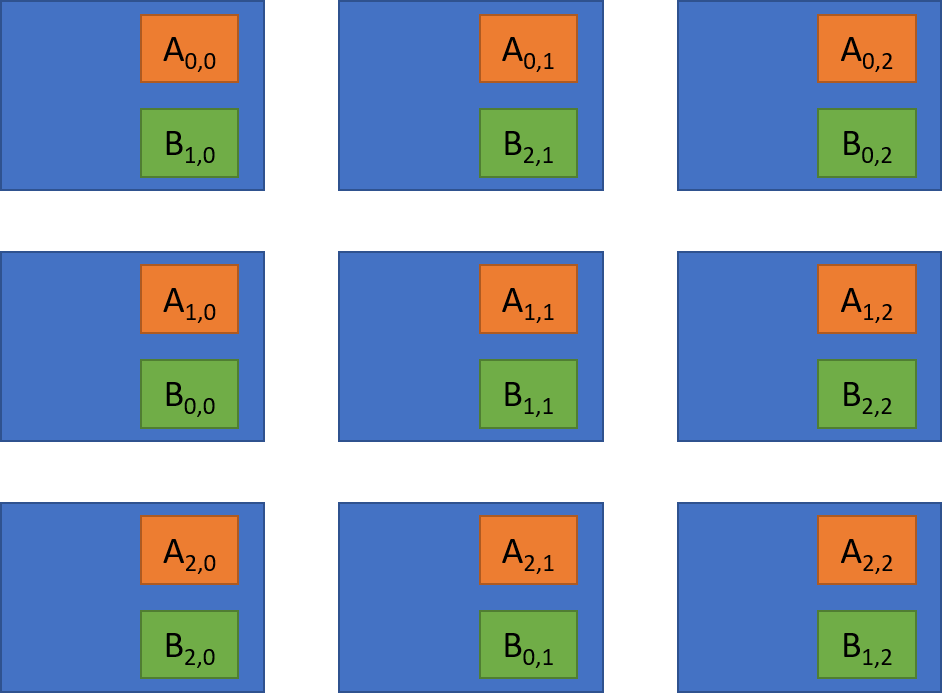
\includegraphics[width=0.72\linewidth]{figures/step_0_cannon.png}
		\caption{Starting Point}
	\end{figure}
\end{frame}

\begin{frame}{Cannon's Algorithm}
	\begin{figure}	
		\centering
		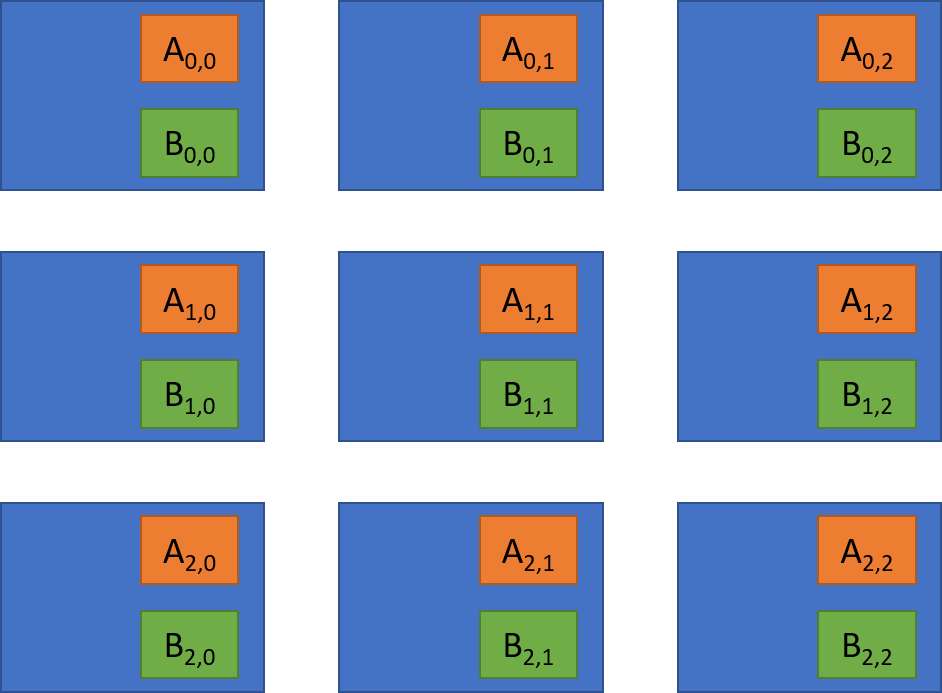
\includegraphics[width=0.72\linewidth]{figures/step_1_cannon.png}
		\caption{Alignment}
	\end{figure}
\end{frame}

\begin{frame}{Cannon's Algorithm}
	\begin{figure}	
		\centering
		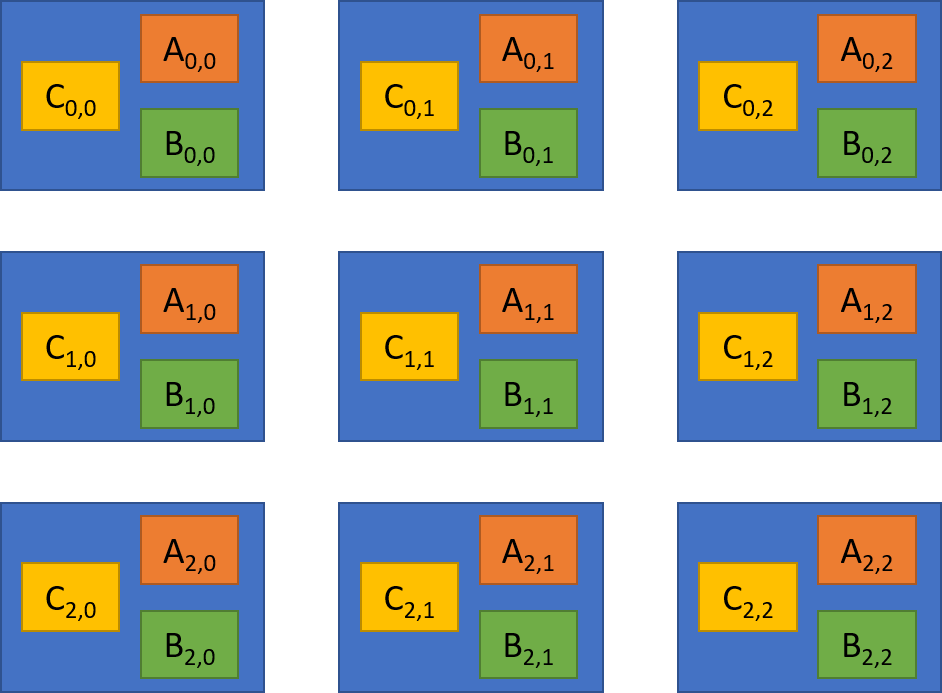
\includegraphics[width=0.72\linewidth]{figures/step_2_cannon.png}
		\caption{Multiply Local Values}
	\end{figure}
\end{frame}

\begin{frame}{Cannon's Algorithm}
\begin{figure}	
	\centering
	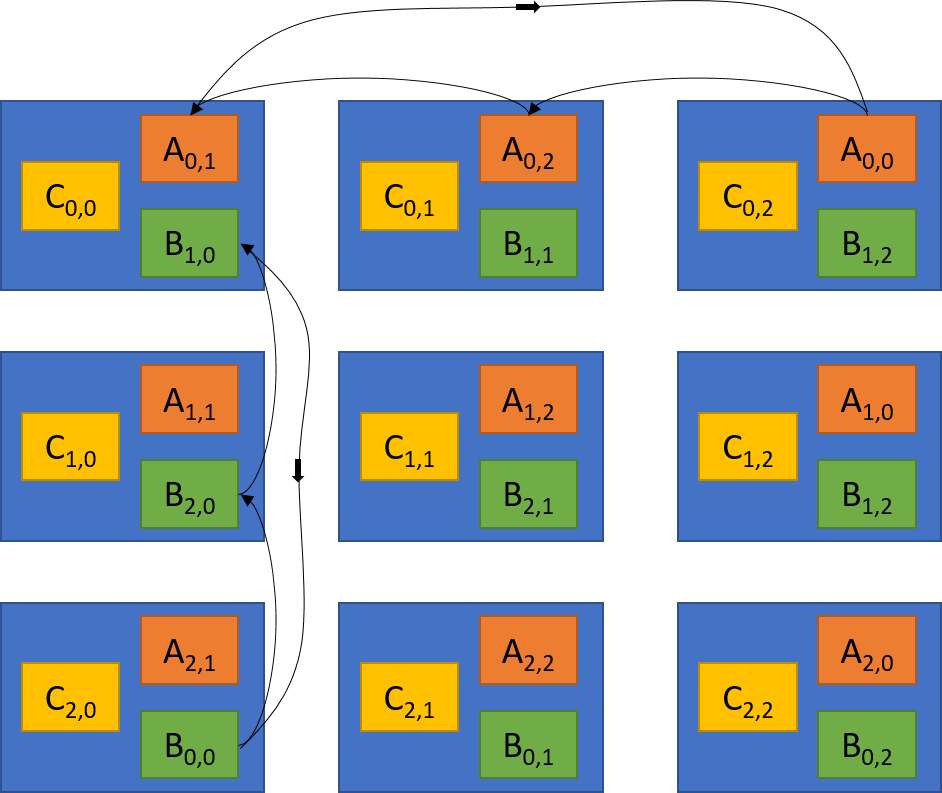
\includegraphics[width=0.72\linewidth]{figures/step_3_cannon.png}
	\caption{Shift Data}
\end{figure}
\end{frame}

\begin{frame}{Cannon's Algorithm}
\begin{figure}	
\centering
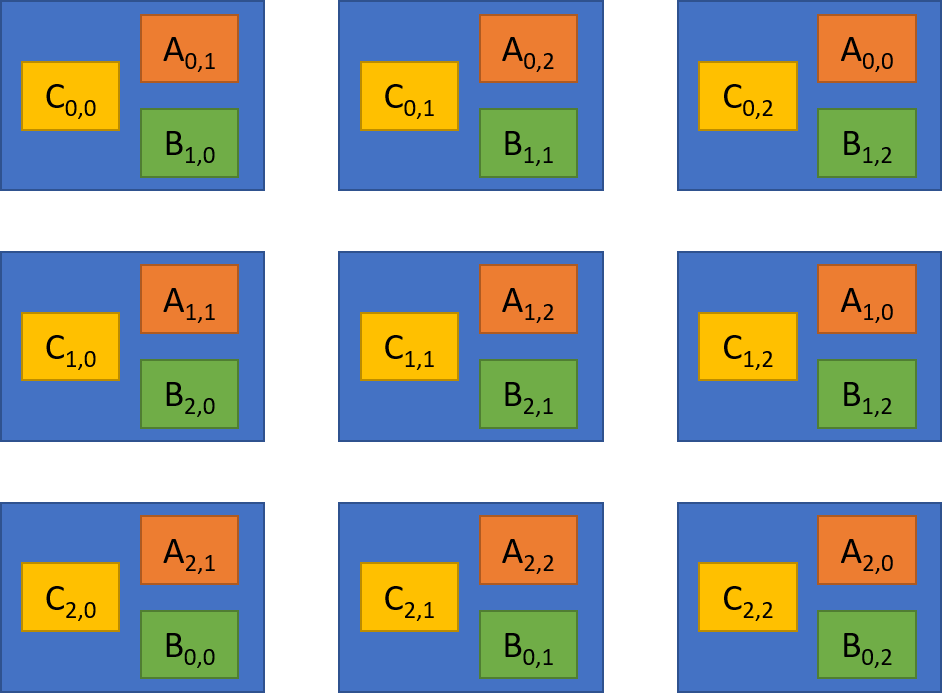
\includegraphics[width=0.72\linewidth]{figures/step_2_cannon_2.png}
\caption{Multiply Local Values}
\end{figure}
\end{frame}

\begin{frame}{Cannon's Algorithm}
\begin{figure}	
	\centering
	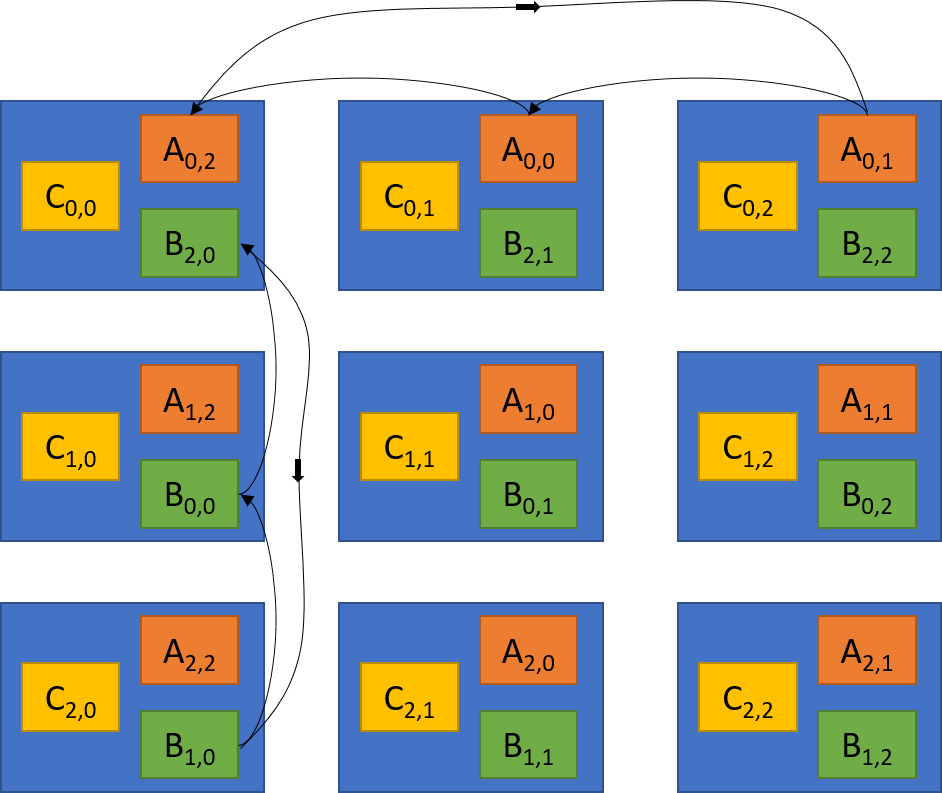
\includegraphics[width=0.72\linewidth]{figures/step_3_cannon_2.png}
	\caption{Shift Data}
\end{figure}
\end{frame}

\begin{frame}{Cannon's Algorithm}
\begin{figure}	
	\centering
	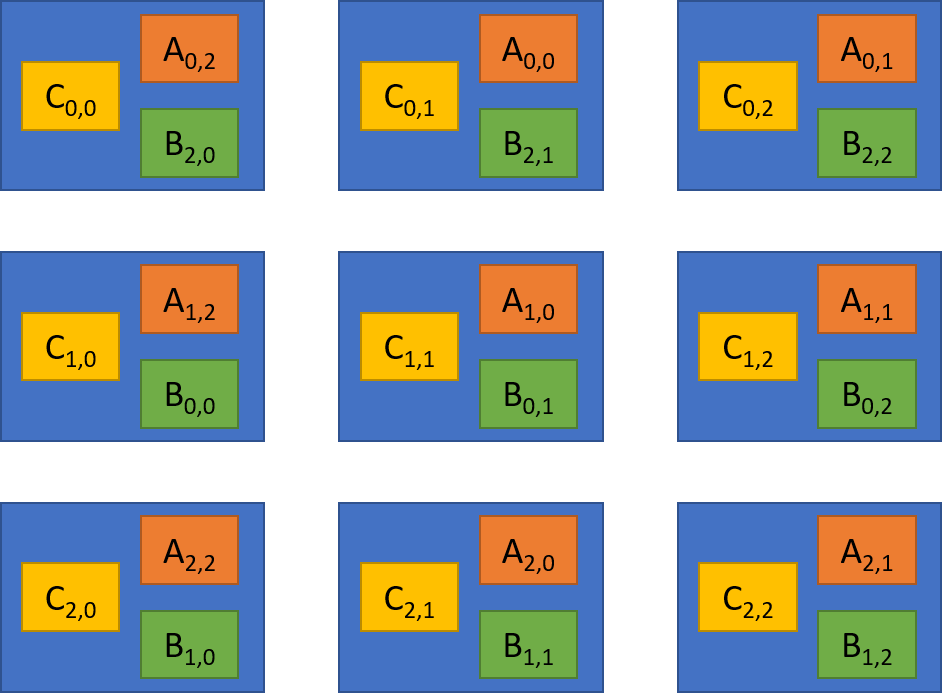
\includegraphics[width=0.72\linewidth]{figures/step_2_cannon_3.png}
	\caption{Multiply Local Values}
\end{figure}
\end{frame}

\begin{frame}{Distributed CSV Read}
\begin{outline}
	\1 Currently no Distributed Data Loading
		\2 Manual specification of data in PhySL strings
	\1 Bottleneck to serious testing
	\1 Simple Fix
		\2 Base off existing CSV read primitive
		\2 Use filename as custom basename for finding participating localities
\end{outline}
\end{frame}

\begin{frame}[standout]
	Questions?
\end{frame}

\end{document}
